\chapter{La Complicaci\'on: Restricci\'on de Estacionalidad en los Campos}

Todas las soluciones anteriores suponen que el agente al final de la cadena (el proveedor de materias primas) tiene inventario infinito. ¿Y si no fuera as\'i?

... que los campos tengan una restricci\'on temporal y solamente produzcan en los ciclos naturales de la cebada

Incluir aqu\'i la imagen de los ciclos naturales de la cebada \ref{fields}

\begin{figure}[h]
\caption{ }
\label{fields}
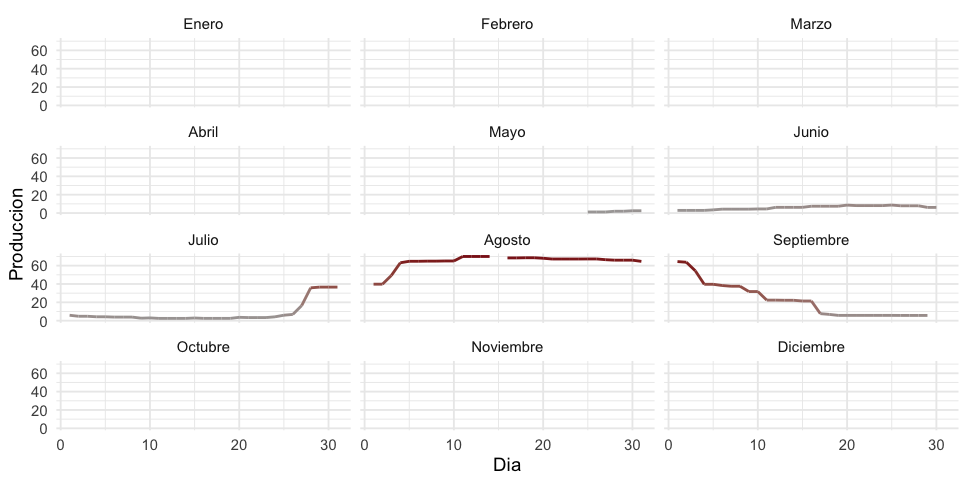
\includegraphics[width=15cm]{fields_monthly_supply_ggplot.png}
\centering
\end{figure}


En este trabajo presentaremos un modelo con esta restricci\'on, lo resolveremos tanto con \textit{policy iteration} como con \textit{Q-learning}
